\clearpage
\SourceLeaf{002}\pdfbookmark[0]{Werke. Siebenter Band}{werke-cover}
\thispagestyle{empty}
\begin{center}
\vspace*{.8in}
{\Large CARL FRIEDRICH GAUSS}\par\bigskip
{\Huge WERKE}\par\bigskip
{\large SIEBENTER BAND}\par\vspace{.6in}
HERAUSGEGEBEN\par\medskip
VON DER\par\bigskip
{\small KÖNIGLICHEN GESELLSCHAFT DER WISSENSCHAFTEN}\par\medskip
ZU\par\bigskip
{\large GÖTTINGEN}\par\vfill
{\small IN COMMISSION BEI B. G. TEUBNER IN LEIPZIG}\par\medskip
1906.
\end{center}
\clearpage
\SourceLeaf{004}\pdfbookmark[1]{Werke. Band VII.}{half-title}
\thispagestyle{empty}
\begin{center}\vspace*{2.3in}
{\Large CARL FRIEDRICH GAUSS WERKE}\par\bigskip
{\large BAND VII.}
\end{center}
\clearpage
\SourceLeaf{006}\pdfbookmark[1]{Werke. Siebenter Band.}{werke-title}
\thispagestyle{empty}
\begin{center}
{\Large CARL FRIEDRICH GAUSS}\par\bigskip
{\Huge WERKE}\par\bigskip
{\large SIEBENTER BAND.}\par\medskip
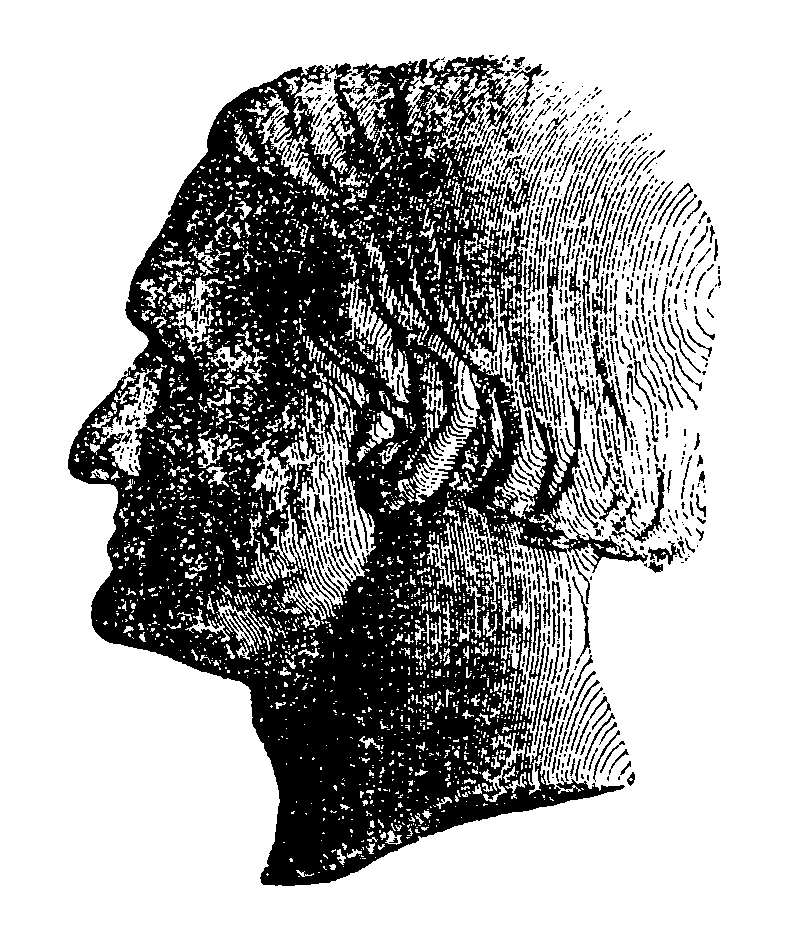
\includegraphics[height=2.05in]{images/gauss_portrait.png}\par\medskip
HERAUSGEGEBEN\par\smallskip
VON DER\par\medskip
{\small KÖNIGLICHEN GESELLSCHAFT DER WISSENSCHAFTEN}\par\smallskip
ZU\par\medskip
{\large GÖTTINGEN.}\par\vfill
{\small IN COMMISSION BEI B. G. TEUBNER IN LEIPZIG.}\par\medskip
1906.
\end{center}
\clearpage
\SourceLeaf{008}\pdfbookmark[0]{Theoria motus corporum coelestium}{theoria-title}
\thispagestyle{empty}
\begin{center}
\vspace*{.3in}
{\LARGE THEORIA}\par\bigskip
{\Large MOTUS CORPORUM}\par\bigskip
{\Large COELESTIUM}\par\bigskip
IN\par\bigskip
{\small SECTIONIBUS CONICIS SOLEM AMBIENTIUM}\par\bigskip
AUCTORE\par\bigskip
{\large CAROLO FRIDERICO GAUSS}\par\bigskip
\rule{.6\linewidth}{.3pt}\par\bigskip
{\small HAMBURGI SUMTIBUS FRID. PERTHES ET I. H. BESSER}\par\medskip
1809.\par\medskip
\rule{.3\linewidth}{.3pt}\par\bigskip
Venditur
\end{center}
{\footnotesize\noindent
\begin{tabular*}{\linewidth}{@{}l@{\extracolsep{\fill}}l@{}}
\textsc{Parisiis} ap. Treuttel \& Würtz. & \textsc{Londini} ap. R. H. Evans.\\
\textsc{Stockholmiae} ap. A. Wiborg. & \textsc{Petropoli} ap. Klostermann.\\
\textsc{Madriti} ap. Sancha. & \textsc{Florentiae} ap. Molini, Landi \& C\raisebox{.2ex}{\scriptsize o}.\\
\end{tabular*}\par\smallskip\noindent
\textsc{Amstelodami} in libraria: Kunst- und Industrie-Comptoir, dicta.\par}
